%!TEX root = prelim.tex

\frame{\frametitle{Compound Effect of Alignment and Illumination}
\renewcommand{\imagesizestring}{height}
\renewcommand{\imagesizea}{0.25\textheight}
\renewcommand{\imagesizeb}{0.15\textheight}
\renewcommand{\gapsizea}{-0mm}
\begin{tabular}[b]{cc@{}b{.5\textwidth}}
% Example for setting the heights of the images
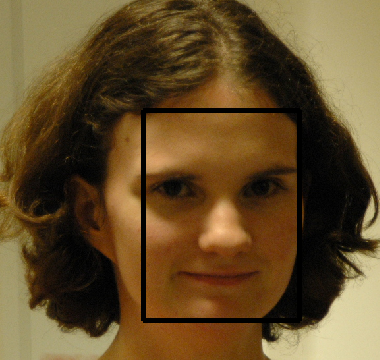
\includegraphics[\imagesizestring=\imagesizea]{figures_cvpr/promo/case1/detector.png}& \hspace{\gapsizea}
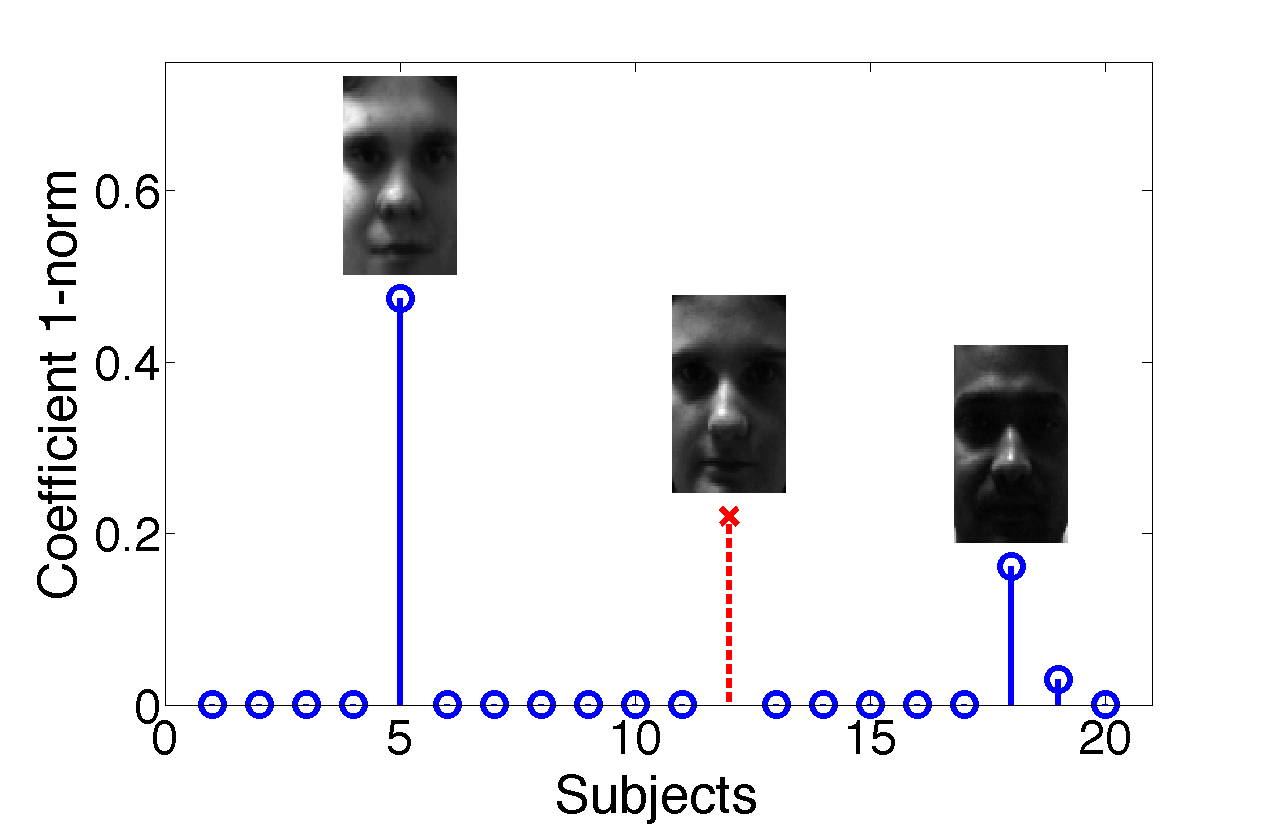
\includegraphics[\imagesizestring=\imagesizea]{figures_cvpr/promo/case1/sci_with_axis_face_case1.png} & 
Poor alignment, {\bf Sufficient training illuminations} \vfill\\
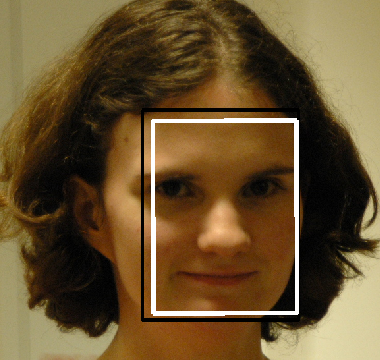
\includegraphics[\imagesizestring=\imagesizea]{figures_cvpr/promo/alignment_and_detector.png}& \hspace{\gapsizea}
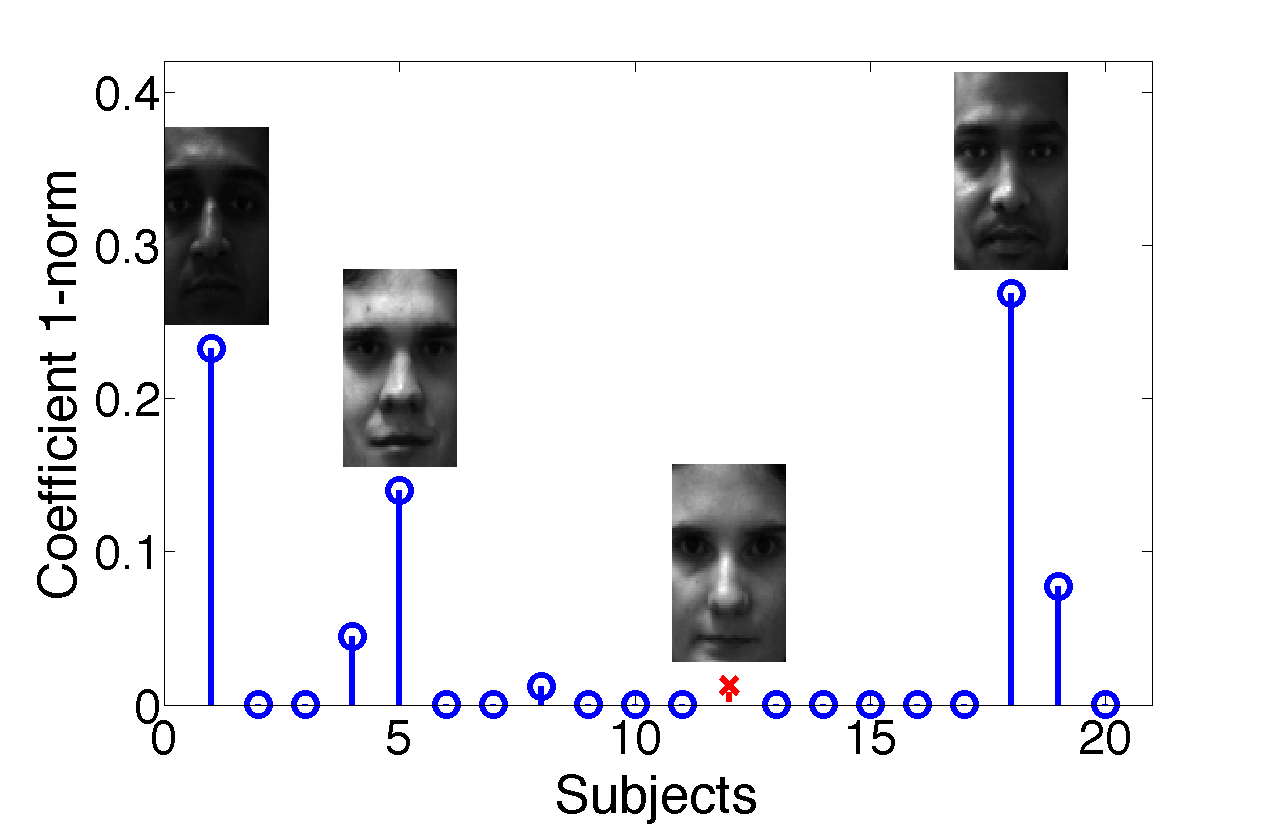
\includegraphics[\imagesizestring=\imagesizea]{figures_cvpr/promo/case2/sci_with_axis_face_case2.png} & 
{Good alignment, {\bf Insufficient training illuminations}}\vfill\\
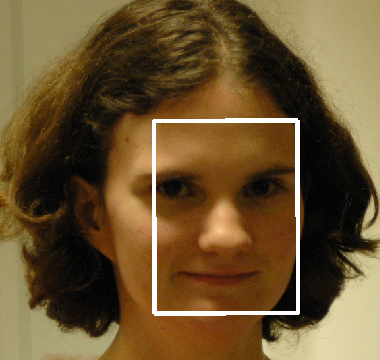
\includegraphics[\imagesizestring=\imagesizea]{figures_cvpr/promo/case3/alignment.png} & \hspace{\gapsizea}
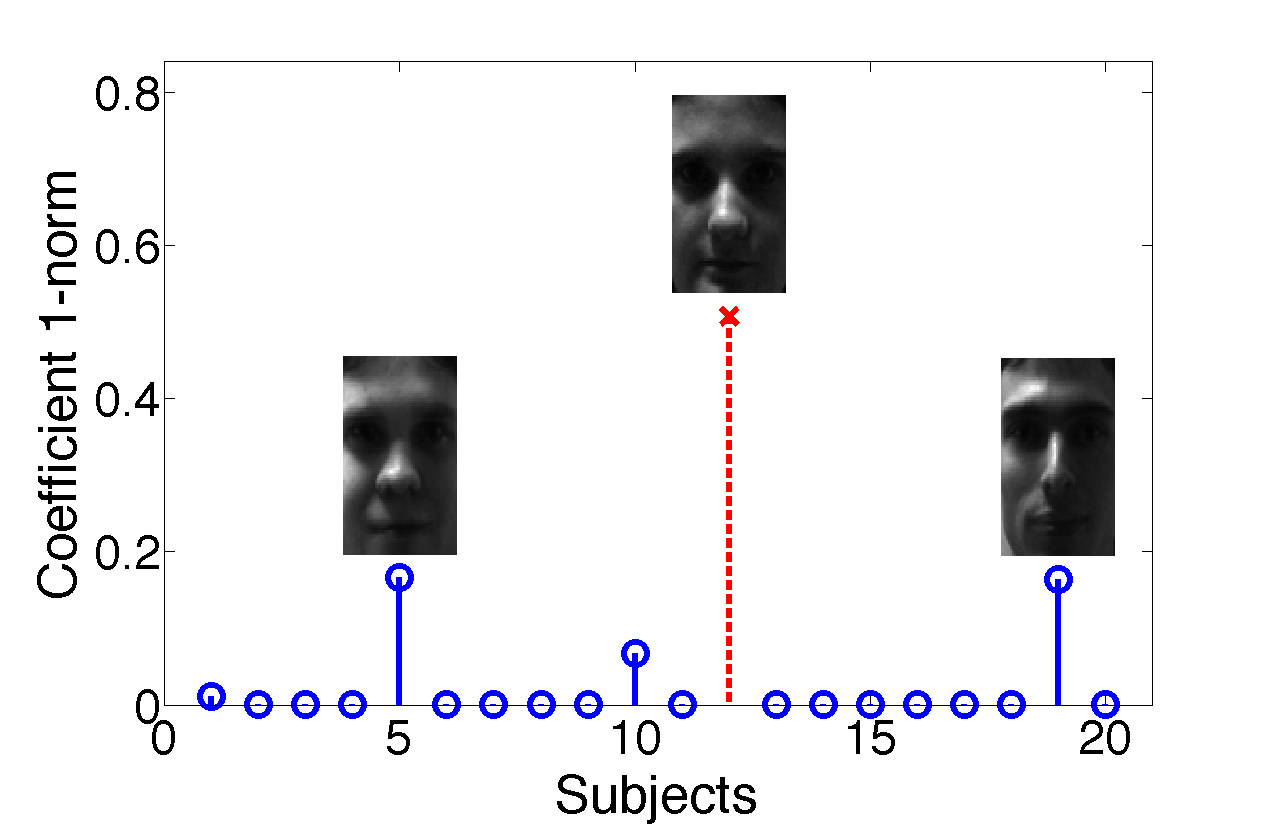
\includegraphics[\imagesizestring=\imagesizea]{figures_cvpr/promo/case3/sci_with_axis_face_case3.png} &
{Good alignment, {\bf Sufficient training illuminations}}\vfill
\end{tabular}
}


\frame{
\frametitle{Linear Illumination Models}
\hspace{.1\textwidth}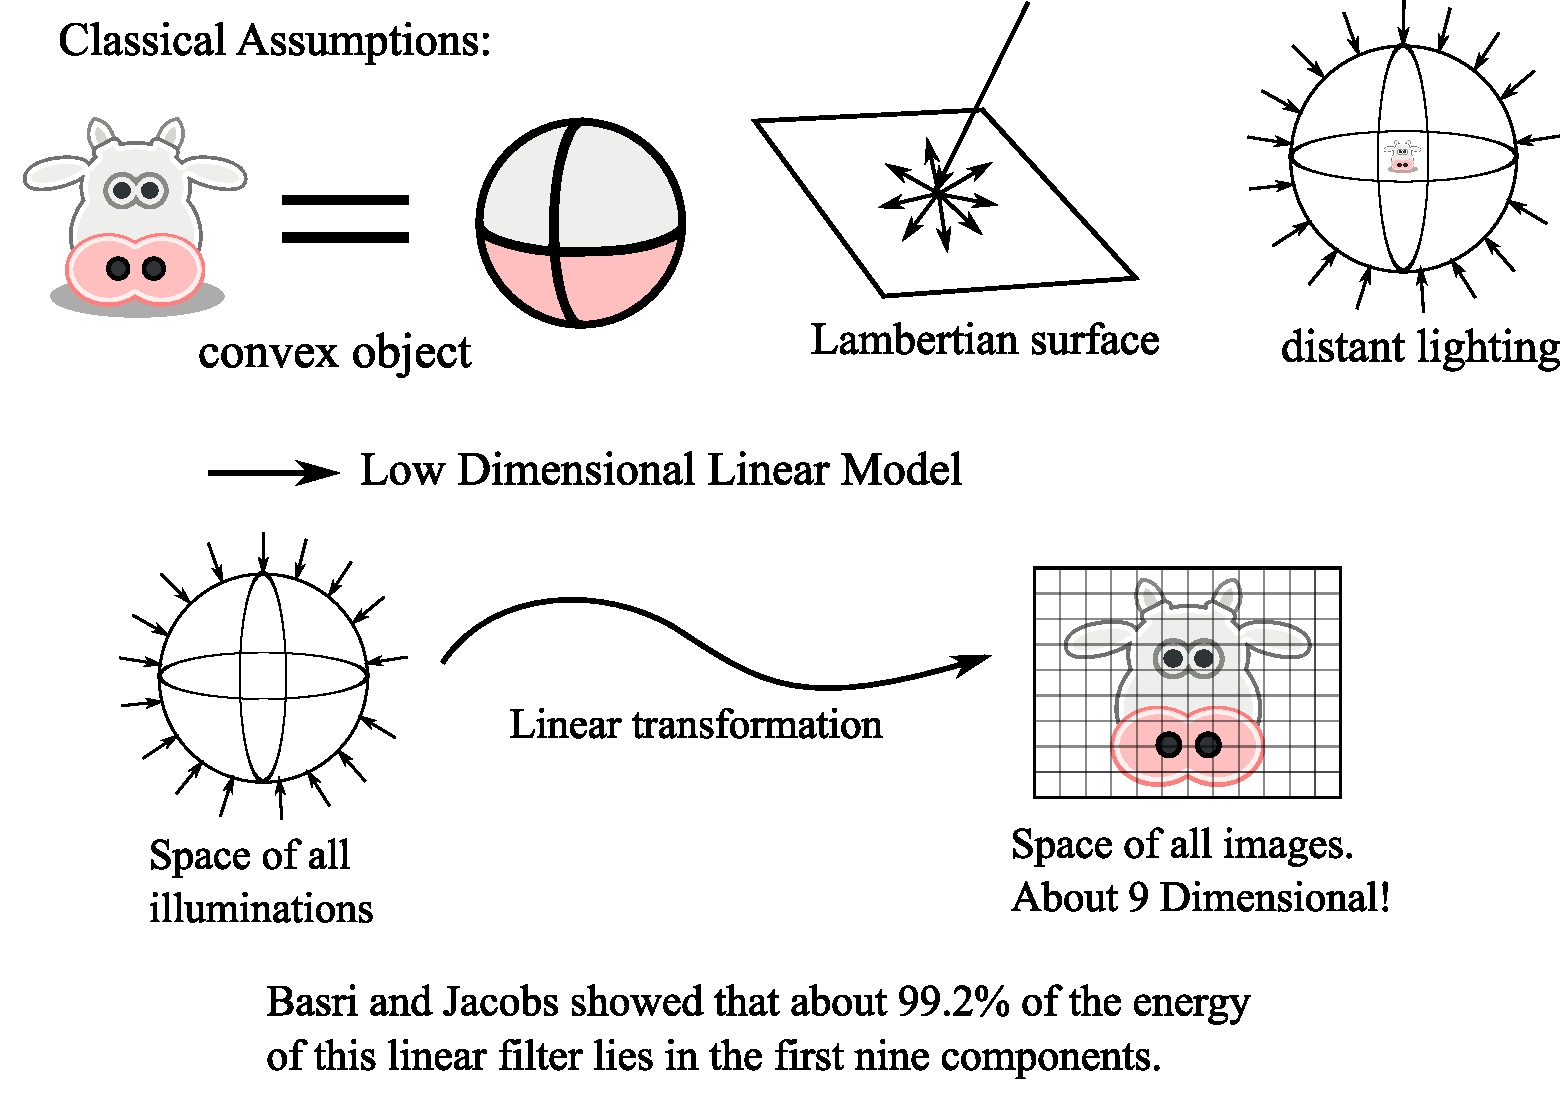
\includegraphics[height=0.8\textheight]{images/linear_illumination_model.pdf}
}

\frame{
\frametitle{Cows are not spherical}
\vspace{-5mm}\begin{center}
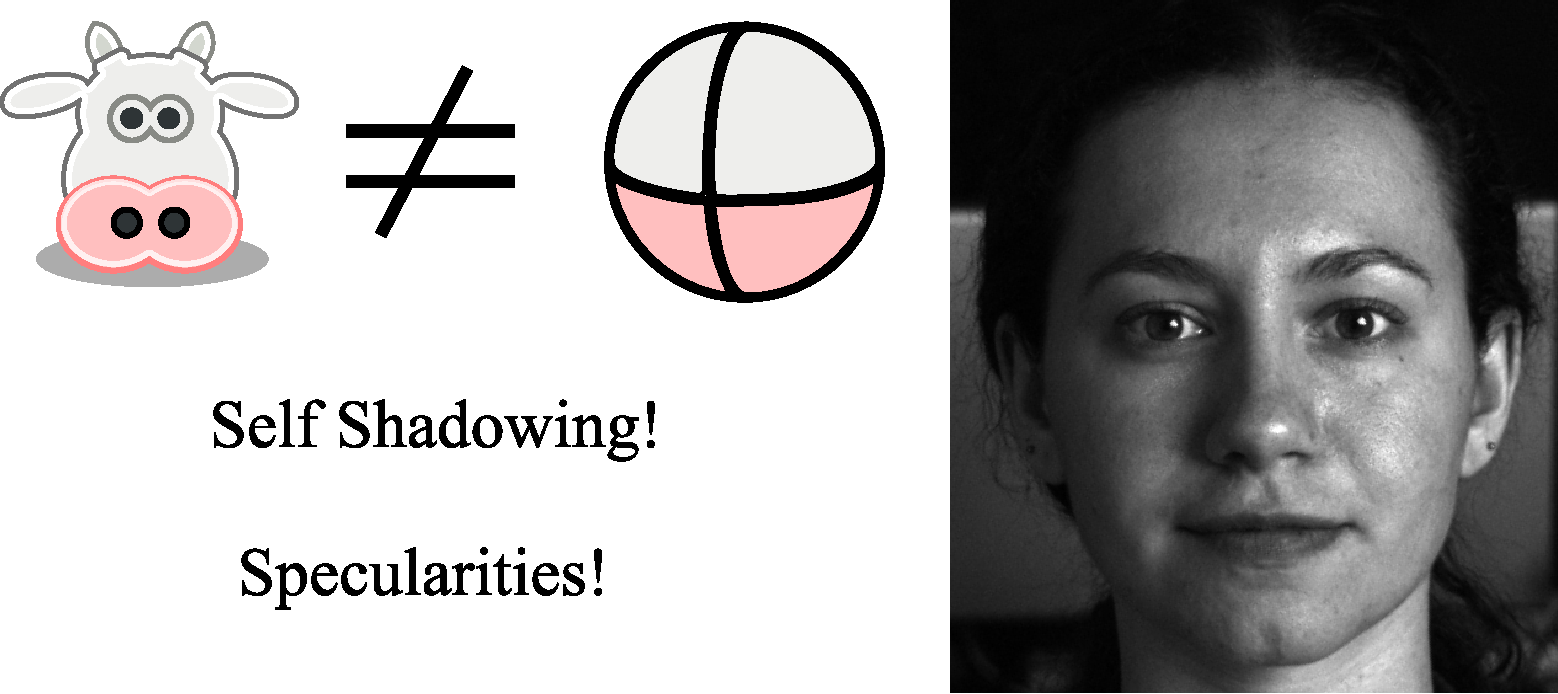
\includegraphics[width=0.9\textwidth]{images/basri4.pdf}
\end{center}\vspace{-5mm}
\begin{itemize}
\item Images still linear WRT illumination
\item {\em Experimentally} determine which training illuminations needed
\end{itemize}
}
